\section{Durchführung}
\label{sec:Durchfuehrung}
\subsection{Vorbereitung}
Als Vorbereitung werden die Energien $E_{\text{K}\alpha}$ und $E_{\text{K}\beta}$ für Kupfer recherchiert.
\begin{align}
    E_{\text{K}\alpha} &= 8,038\text{keV}    &&   E_{\text{K}\beta} = 8,905\text{keV} \label{eqn:EnergieKupfer}
\end{align}
Und es werden die entsprechenden Wellenlängen für die Energien berechnet.
\begin{align}
    E &= \frac{h\cdot c}{\lambda} && \lambda = \frac{h\cdot c}{E} \nonumber \\
    \lambda_{\text{K}\alpha} &= 2,471\cdot 10^{-29} \text{m} \\
    \lambda_{\text{K}\beta} &= 2,231 \cdot 10^{-29} \text{m} 
\end{align}
Über den Sinus werden aus den Wellenlängen die entsprechenden Glanzwinkel berechnet.
\begin{align}
   2d\sin{\alpha} &= n\lambda && \alpha = \arcsin \left(\frac{n\lambda}{2d}\right) \nonumber \\
   \alpha_{\text{K}\alpha} &= 6,135° \cdot 10^{-20} \\
   \alpha_{\text{K}\beta} &= 5,538° \cdot 10^{-20}
\end{align}
Außerdem wird als Referenz die Comptonwellenlänge des Elektrons theoretisch berechnet.
\begin{equation}
    \lambda_{\text{C}} = \frac{h}{m_e c} = 2,42631 \cdot 10^{-12} \text{m}
\end{equation}



\subsection{Versuch}
\subsubsection{Charakteristische Strahlung von Kupfer}
Aus den Kupfer Messwerten bildet sich:
\begin{figure}[H]
    \centering
    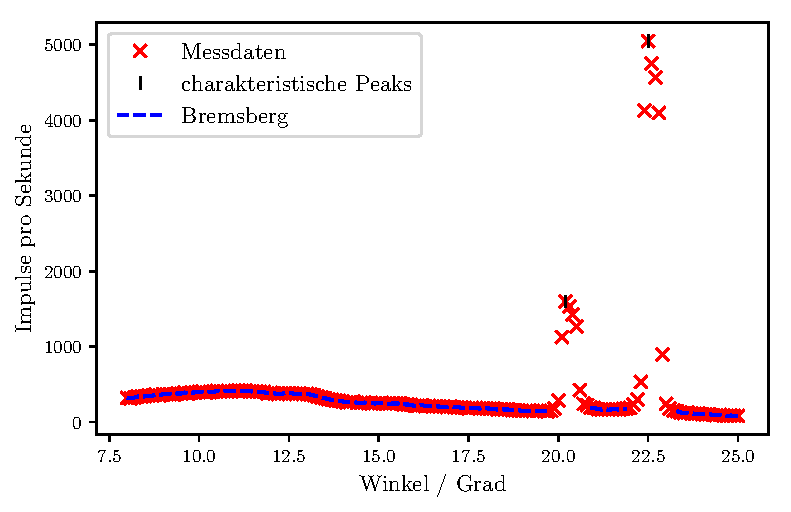
\includegraphics[width=0.7\textwidth]{plots/CU_Spektrum.pdf}
    \caption{Kupfer Emissionsspektrum mit Peaks und Bremsberg}
    \label{fig:CU_Spektrum}
\end{figure}
Mit den Peaks bei 1599 Impulsen pro Sekunde bei 20,2° und 5050 Impulsen pro Sekunde bei 22,5°.
Über die abgelesenen Winkel an den Peaks lassen sich nun die entsprechenden Energien berechnen.


\subsubsection{Compton Wellenlänge}
Es wird die Transmission von Aluminium gemessen.
